% Options for packages loaded elsewhere
\PassOptionsToPackage{unicode}{hyperref}
\PassOptionsToPackage{hyphens}{url}
%
\documentclass[
]{article}
\usepackage{amsmath,amssymb}
\usepackage{iftex}
\ifPDFTeX
  \usepackage[T1]{fontenc}
  \usepackage[utf8]{inputenc}
  \usepackage{textcomp} % provide euro and other symbols
\else % if luatex or xetex
  \usepackage{unicode-math} % this also loads fontspec
  \defaultfontfeatures{Scale=MatchLowercase}
  \defaultfontfeatures[\rmfamily]{Ligatures=TeX,Scale=1}
\fi
\usepackage{lmodern}
\ifPDFTeX\else
  % xetex/luatex font selection
\fi
% Use upquote if available, for straight quotes in verbatim environments
\IfFileExists{upquote.sty}{\usepackage{upquote}}{}
\IfFileExists{microtype.sty}{% use microtype if available
  \usepackage[]{microtype}
  \UseMicrotypeSet[protrusion]{basicmath} % disable protrusion for tt fonts
}{}
\makeatletter
\@ifundefined{KOMAClassName}{% if non-KOMA class
  \IfFileExists{parskip.sty}{%
    \usepackage{parskip}
  }{% else
    \setlength{\parindent}{0pt}
    \setlength{\parskip}{6pt plus 2pt minus 1pt}}
}{% if KOMA class
  \KOMAoptions{parskip=half}}
\makeatother
\usepackage{xcolor}
\usepackage{color}
\usepackage{fancyvrb}
\newcommand{\VerbBar}{|}
\newcommand{\VERB}{\Verb[commandchars=\\\{\}]}
\DefineVerbatimEnvironment{Highlighting}{Verbatim}{commandchars=\\\{\}}
% Add ',fontsize=\small' for more characters per line
\newenvironment{Shaded}{}{}
\newcommand{\AlertTok}[1]{\textcolor[rgb]{1.00,0.00,0.00}{\textbf{#1}}}
\newcommand{\AnnotationTok}[1]{\textcolor[rgb]{0.38,0.63,0.69}{\textbf{\textit{#1}}}}
\newcommand{\AttributeTok}[1]{\textcolor[rgb]{0.49,0.56,0.16}{#1}}
\newcommand{\BaseNTok}[1]{\textcolor[rgb]{0.25,0.63,0.44}{#1}}
\newcommand{\BuiltInTok}[1]{\textcolor[rgb]{0.00,0.50,0.00}{#1}}
\newcommand{\CharTok}[1]{\textcolor[rgb]{0.25,0.44,0.63}{#1}}
\newcommand{\CommentTok}[1]{\textcolor[rgb]{0.38,0.63,0.69}{\textit{#1}}}
\newcommand{\CommentVarTok}[1]{\textcolor[rgb]{0.38,0.63,0.69}{\textbf{\textit{#1}}}}
\newcommand{\ConstantTok}[1]{\textcolor[rgb]{0.53,0.00,0.00}{#1}}
\newcommand{\ControlFlowTok}[1]{\textcolor[rgb]{0.00,0.44,0.13}{\textbf{#1}}}
\newcommand{\DataTypeTok}[1]{\textcolor[rgb]{0.56,0.13,0.00}{#1}}
\newcommand{\DecValTok}[1]{\textcolor[rgb]{0.25,0.63,0.44}{#1}}
\newcommand{\DocumentationTok}[1]{\textcolor[rgb]{0.73,0.13,0.13}{\textit{#1}}}
\newcommand{\ErrorTok}[1]{\textcolor[rgb]{1.00,0.00,0.00}{\textbf{#1}}}
\newcommand{\ExtensionTok}[1]{#1}
\newcommand{\FloatTok}[1]{\textcolor[rgb]{0.25,0.63,0.44}{#1}}
\newcommand{\FunctionTok}[1]{\textcolor[rgb]{0.02,0.16,0.49}{#1}}
\newcommand{\ImportTok}[1]{\textcolor[rgb]{0.00,0.50,0.00}{\textbf{#1}}}
\newcommand{\InformationTok}[1]{\textcolor[rgb]{0.38,0.63,0.69}{\textbf{\textit{#1}}}}
\newcommand{\KeywordTok}[1]{\textcolor[rgb]{0.00,0.44,0.13}{\textbf{#1}}}
\newcommand{\NormalTok}[1]{#1}
\newcommand{\OperatorTok}[1]{\textcolor[rgb]{0.40,0.40,0.40}{#1}}
\newcommand{\OtherTok}[1]{\textcolor[rgb]{0.00,0.44,0.13}{#1}}
\newcommand{\PreprocessorTok}[1]{\textcolor[rgb]{0.74,0.48,0.00}{#1}}
\newcommand{\RegionMarkerTok}[1]{#1}
\newcommand{\SpecialCharTok}[1]{\textcolor[rgb]{0.25,0.44,0.63}{#1}}
\newcommand{\SpecialStringTok}[1]{\textcolor[rgb]{0.73,0.40,0.53}{#1}}
\newcommand{\StringTok}[1]{\textcolor[rgb]{0.25,0.44,0.63}{#1}}
\newcommand{\VariableTok}[1]{\textcolor[rgb]{0.10,0.09,0.49}{#1}}
\newcommand{\VerbatimStringTok}[1]{\textcolor[rgb]{0.25,0.44,0.63}{#1}}
\newcommand{\WarningTok}[1]{\textcolor[rgb]{0.38,0.63,0.69}{\textbf{\textit{#1}}}}
\usepackage{graphicx}
\makeatletter
\def\maxwidth{\ifdim\Gin@nat@width>\linewidth\linewidth\else\Gin@nat@width\fi}
\def\maxheight{\ifdim\Gin@nat@height>\textheight\textheight\else\Gin@nat@height\fi}
\makeatother
% Scale images if necessary, so that they will not overflow the page
% margins by default, and it is still possible to overwrite the defaults
% using explicit options in \includegraphics[width, height, ...]{}
\setkeys{Gin}{width=\maxwidth,height=\maxheight,keepaspectratio}
% Set default figure placement to htbp
\makeatletter
\def\fps@figure{htbp}
\makeatother
\setlength{\emergencystretch}{3em} % prevent overfull lines
\providecommand{\tightlist}{%
  \setlength{\itemsep}{0pt}\setlength{\parskip}{0pt}}
\setcounter{secnumdepth}{-\maxdimen} % remove section numbering
\ifLuaTeX
  \usepackage{selnolig}  % disable illegal ligatures
\fi
\IfFileExists{bookmark.sty}{\usepackage{bookmark}}{\usepackage{hyperref}}
\IfFileExists{xurl.sty}{\usepackage{xurl}}{} % add URL line breaks if available
\urlstyle{same}
\hypersetup{
  hidelinks,
  pdfcreator={LaTeX via pandoc}}

\author{}
\date{}

\usepackage{ctex}
\usepackage{geometry}
\usepackage{titlesec}
\usepackage{float}
\geometry{a4paper, left=2cm, right=2cm, top=2cm, bottom=2cm}
\titleformat{\section}{\normalfont\fontsize{14}{15}\bfseries}{\thesection}{1em}{}

\begin{document}
\title{Link Prediction实验}
\author{211250109 赵政杰}
\date{\today}
\maketitle
复现论文:\href{https://arxiv.org/pdf/2308.16469v2.pdf}{Link Prediction for Wikipedia Articles as a Natural Language Inference Task}
\section{1.论文摘要abstract和introduction翻译}\label{1ux8bbaux6587ux6458ux8981abstractux548cintroductionux7ffbux8bd1}

\subsection{abstract译文}\label{abstractux8bd1ux6587}

链接预测任务(link prediction task)对于自动理解大型知识库的结构至关重要。在本文中,我们在 2023
年数据科学和高级分析竞赛(DSAA-2023 Competition)“高效且有效的链接预测”任务中展示了解决此问题的系统,该系统包含
948,233 个训练数据和 238,265 个用于公共测试的语料库。本文介绍了一种在维基百科文章中进行链接预测的方法,将其表述为自然语言推理(NLI)任务。受自然语言处理和理解领域最新进展的启发,我们将链接预测作为一项
NLI 任务,其中两篇文章之间存在链接被视为前提,任务是根据文章中的信息确定该前提是否成立。我们基于维基百科文章的链接预测任务的句对分类来实现我们的系统。我们的系统在公共和私人测试集上分别获得了
0.99996 Macro F1-score 和 1.00000 Macro F1-score。我们 UIT-NLP 团队在私人测试集上的表现排名第三,与第一名和第二名的成绩持平。我们的代码是公开的,用于研究目的。

\subsection{introduction译文}\label{introductionux8bd1ux6587}

维基百科(Wikipedia)是世界上最大的协作式百科全书,已成为获取各种主题知识的宝贵资源。维基百科拥有数百万篇涵盖不同主题的文章,提供了一个不断扩展的庞大信息库。然而,尽管维基百科的规模令人印象深刻,但维基百科的文章之间的相互链接并不总是全面的,导致信息连通性方面存在差距。

链接预测是网络分析中的一项基本任务,旨在根据现有连接预测给定网络中缺失的链接。在维基百科的背景下,链接预测变得尤为重要,因为它可以帮助增强百科全书的导航性、提高信息可访问性并促进对相关主题的更深入理解。
DSAA-2023
挑战赛重点关注应用于维基百科文章的链接预测任务。此外,DSAA-2023
挑战赛的重点是提出类网络数据结构中的链路预测方法,例如网络重建和网络开发,使用维基百科文章作为主要数据源。

自然语言推理的任务是在给定“前提”的情况下确定“假设”是真(蕴含)、假(矛盾)还是不确定(中性)。
维基百科文章任务的链接预测被定义为给出维基百科网络的稀疏子图并预测两个维基百科页面之间是否存在链接。
在本文中,我们利用自然语言推理任务和维基百科文章的链接预测任务之间固有的相似性,将
NLI 中常用的句对分类 (SPC) 技术应用于链接预测任务的特定上下文。

本文通过结合基于 NLI 的 SPC
和预处理技术来解决维基百科文章的链接预测挑战。维基百科中链接预测的传统方法通常依赖于基于图的算法或文本相似性度量,这可能会忽略文章文本中嵌入的微妙关系。通过集成句对分类和预处理技术,我们旨在更有效地捕获维基百科文章中的语义和上下文信息,以提高链接预测准确性。

我们的贡献总结如下:

\begin{enumerate}
  \def\labelenumi{\arabic{enumi}.}
  \item
        首先,我们采用高效的数据预处理技术来清洗从维基百科获得的评论。这些技术的利用有助于提高数据的整体质量,并在为链接预测任务训练模型之前改进相关信息的提取。
  \item
        其次,我们通过将 NLI
        与维基百科文章的链接预测之间的相似性结合起来,采用了自然语言推理中广泛使用的
        SPC 技术来进行链接预测。
  \item
        最后,我们在这项任务上取得了最好的成绩,在公开测试中得分为
        0.99996,在私人测试中得分为 1.00000 ,分别排名第八和第三。
\end{enumerate}

\section{2.问题描述}\label{2ux95eeux9898ux63cfux8ff0}

维基百科文章链接预测任务是指基于给定的维基百科数据集,预测一对文章节点
(u, v)
之间是否存在边。更准确地说,给定维基百科文章网络的稀疏子图,确定维基百科上下文中两个页面
u 和 v 之间是否存在链接。

\section{3.输入、输出、模型算法描述}\label{3ux8f93ux5165ux8f93ux51faux6a21ux578bux7b97ux6cd5ux63cfux8ff0}

\subsection{输入}\label{ux8f93ux5165}

\begin{enumerate}
  \def\labelenumi{\arabic{enumi}.}
  \item
        train.csv文件:它包含节点对以及它们之间是否存在边的label。该文件有四列:id、id1、id2
        和 label。id 列表示配对标识符,id1 和 id2 是文章节点标识符,label
        表示两节点之间是否存在边(0或1)。
  \item
        nodes.zip文件:此文件是 nodes.tsv
        的压缩版本,包含每个文章节点的信息。它由两列组成:id(文章节点标识符)
        和 text (节点的文本描述)。
\end{enumerate}

\subsection{输出}\label{ux8f93ux51fa}

输出模型的预测结果,输出格式参照
sample\_submission.csv,应当包含两类,一列是 pair
ID,即配对标识符;一列为 label,表示两节点是否存在边(0或1)。

\subsection{模型算法描述}\label{ux6a21ux578bux7b97ux6cd5ux63cfux8ff0}

\subsubsection{方法架构图}\label{ux65b9ux6cd5ux67b6ux6784ux56fe}

\begin{figure}[H]
  \centering
  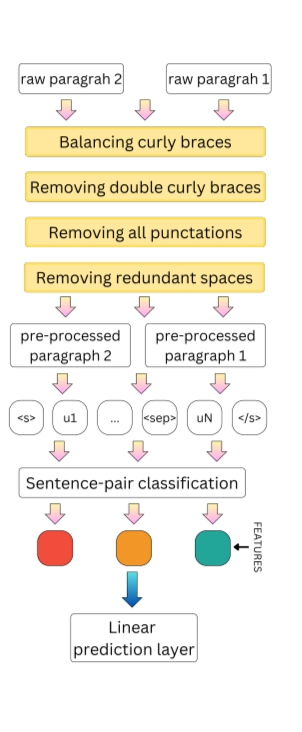
\includegraphics[height=0.4\textheight]{./pic/1.png}
\end{figure}

\subsubsection{预处理算法}\label{ux9884ux5904ux7406ux7b97ux6cd5}

该数据集由维基百科对象的主要内容和维基百科内的 CSS 代码组成。然而,这些
CSS 代码被认为是噪声,不需要进行训练。因此,去除它们至关重要。
为了实现这一目标,我们采用两种算法,即平衡花括号算法和删除双花括号算法。

\begin{enumerate}
  \def\labelenumi{\arabic{enumi}.}
  \item
        \textbf{平衡花括号算法}(Balancing Curly Braces)

        算法步骤:

        \begin{enumerate}
          \def\labelenumii{\arabic{enumii}.}
          \item
                分别统计左花括号和右花括号的数量,并将结果存储在\texttt{opening\_count}和\texttt{closing\_count}变量中。
          \item
                平衡花括号:

                \begin{itemize}
                  \item
                        如果\texttt{opening\_count}大于\texttt{closing\_count},说明需要删除一些左花括号。

                        \begin{itemize}
                          \item
                                进入一个\texttt{while}循环,条件是\texttt{opening\_count}大于\texttt{closing\_count}。
                          \item
                                删除找到的第一个左花括号,将\texttt{opening\_count}减1。
                          \item
                                重复此过程,直到左右花括号相等。
                        \end{itemize}
                  \item
                        如果\texttt{closing\_count}大于\texttt{opening\_count},说明需要删除一些右花括号。

                        \begin{itemize}
                          \item
                                进入一个\texttt{while}循环,条件是\texttt{closing\_count}大于\texttt{opening\_count}。
                          \item
                                删除找到的第一个右花括号,将\texttt{closing\_count}减1。
                          \item
                                重复此过程,直到左右花括号相等。
                        \end{itemize}
                \end{itemize}
          \item
                返回平衡后的文本。
        \end{enumerate}

        \begin{Shaded}
          \begin{Highlighting}[]
            \NormalTok{procedure BALANCECURLYBRACES(text)}
            \NormalTok{	opening\_count ← text.count(\textquotesingle{}\{\textquotesingle{})}
            \NormalTok{	closing\_count ← text.count(\textquotesingle{}\}\textquotesingle{})}
            \NormalTok{	if opening\_count \textgreater{} closing\_count then}
            \NormalTok{		while opening\_count \textgreater{} closing\_count do}
            \NormalTok{			index ← text.find(\textquotesingle{}\{\textquotesingle{})}
            \NormalTok{			if index ≠ −1 then}
            \NormalTok{				text = text[:index] + text[index + 1:]}
            \NormalTok{				opening\_count ← opening\_count − 1}
            \NormalTok{	else if closing\_count \textgreater{} opening\_count then}
            \NormalTok{		while closing\_count \textgreater{} opening\_count do}
            \NormalTok{			index ← text.rfind(\textquotesingle{}\}\textquotesingle{})}
            \NormalTok{			if index ≠ −1 then}
            \NormalTok{				text = text[:index] + text[index + 1:]}
            \NormalTok{				closing\_count ← closing\_count − 1}
            \NormalTok{	return text.strip()}
          \end{Highlighting}
        \end{Shaded}
  \item
        \textbf{删除双花括号算法}(Remove Double Curly Braces)

        算法步骤:

        \begin{enumerate}
          \def\labelenumii{\arabic{enumii}.}
          \item
                创建一个空栈\texttt{stack}和一个空字符串\texttt{clean\_text}。
          \item
                遍历文本字符

                \begin{itemize}
                  \item
                        如果是左花括号,则进行压栈。
                  \item
                        如果是右花括号

                        \begin{itemize}
                          \item
                                如果栈非空且栈顶为左花括号,则将其弹栈。
                        \end{itemize}
                  \item
                        如果是其他字符,如果栈为空,则将其添加到\texttt{clean\_text}中。
                \end{itemize}
          \item
                返回去除双花括号后的\texttt{clean\_text}。
        \end{enumerate}

        \begin{Shaded}
          \begin{Highlighting}[]
            \NormalTok{procedure REMOVEDOUBLECURLYBRACES(text)}
            \NormalTok{	stack ← []}
            \NormalTok{	clean\_text ← \textquotesingle{}\textquotesingle{}}
            \NormalTok{	for char in text do}
            \NormalTok{		if char = \textquotesingle{}\{\textquotesingle{} then}
            \NormalTok{			stack.push(char)}
            \NormalTok{		else if char = \textquotesingle{}\}\textquotesingle{} then}
            \NormalTok{			if not isEmpty(stack) and}
            \NormalTok{				top(stack) = \textquotesingle{}\{\textquotesingle{} then}
            \NormalTok{				stack.pop(stack)}
            \NormalTok{		else}
            \NormalTok{			if isEmpty(stack) then}
            \NormalTok{				clean\_text ← clean\_text + char}
            \NormalTok{	return clean\_text}
          \end{Highlighting}
        \end{Shaded}
  \item
        \textbf{利用正则表达式库删除所有标点符号以及冗余空格}
\end{enumerate}

\subsubsection{模型算法}\label{ux6a21ux578bux7b97ux6cd5}

利用自然语言推理任务和维基百科文章的链接预测任务之间固有的相似性,实现了基于XLM-Roberta的句对分类模型来进行链接预测。

模型算法步骤:

\begin{enumerate}
  \def\labelenumi{\arabic{enumi}.}
  \item
        \textbf{分词(Tokenization)}

        \begin{itemize}
          \item
                XLM-Roberta首先接受多语言文本作为输入,并使用分词器将文本分割成离散的tokens(标记)。Tokens
                可以是单词、子词(如词根或词缀)、标点符号等,取决于分词器和分词规则。
        \end{itemize}
  \item
        \textbf{建立Transformer模型}

        \begin{itemize}
          \item
                XLM-Roberta构建在Transformer架构之上。Transformer是一种深度学习模型,特别适用于处理序列数据。
          \item
                模型包括多个Transformer层,每个层都包括多头自注意力机制和前馈神经网络。
          \item
                这些Transformer层通过堆叠来构建深度神经网络,用于学习文本的表示。
        \end{itemize}
  \item
        \textbf{预处理(Pretraining)}

        \begin{itemize}
          \item
                在预训练阶段,XLM-Roberta使用大规模的多语言文本数据进行训练,执行通常是建立“掩盖语言模型”的任务。
          \item
                在掩盖语言模型中,模型被要求预测每个token中一小部分被随机遮盖的部分,以从上下文中理解其含义。
        \end{itemize}
  \item
        \textbf{微调(Fine-tuning)}

        \begin{itemize}
          \item
                预训练完成后,XLM-Roberta可以通过微调来适应特定的下游NLP任务,如文本分类、命名实体识别、文本翻译等。
          \item
                微调通常包括在模型的顶部添加适当的输出层,以匹配任务的类别数或标签,然后进行有监督的训练。

                在此任务中,我们为模型整合了一个线性预测层来计算最终的输出。
          \item
                在微调过程中,模型的参数会针对具体任务的数据集进行调整,以适应任务的需求。
        \end{itemize}
  \item
        \textbf{应用}

        \begin{itemize}
          \item
                将经过微调的XLM-Roberta模型用于链接预测任务,来判断两篇文章之间是否具有关联。
        \end{itemize}
\end{enumerate}

\section{4.评价指标及其计算公式}\label{4ux8bc4ux4ef7ux6307ux6807ux53caux5176ux8ba1ux7b97ux516cux5f0f}

使用\textbf{宏平均F1分数}(Macro F1-score)进行结果的评估。

计算公式如下:

\[\text{Macro F1-score} = \frac{1}{N} \sum_{i=1}^{N} \frac{2 \cdot \text{Precision}_i \cdot \text{Recall}_i}{\text{Precision}_i + \text{Recall}_i}\]

其中:

\begin{itemize}
  \item
        \emph{N} 是类别(链接类型)的总数。在此任务中为2。
  \item
        ${\text{Precision}_i}$是第\emph{i}个类别的精确度(Precision),定义为模型正确预测为该类别的文章对数目除以总的预测为该类别的文章对数目。
  \item
        ${\text{Recall}_i}$是第\emph{i}个类别的召回率(Recall),定义为模型正确预测为该类别的文章对数目除以总的真实属于该类别的文章对数目。
\end{itemize}

上述公式计算了每个类别的F1分数,然后对所有类别的F1分数取平均值,得到宏平均F1分数。这个指标用于综合评估模型在多类别分类任务中的性能,而不受类别不平衡的影响。

\section{5.对比方法及这些对比方法的引用论文出处}\label{5ux5bf9ux6bd4ux65b9ux6cd5ux53caux8fd9ux4e9bux5bf9ux6bd4ux65b9ux6cd5ux7684ux5f15ux7528ux8bbaux6587ux51faux5904}

本文通过结合基于 NLI 的 SPC
和预处理技术来解决维基百科文章的链接预测挑战。

对比传统方法,它们通常依赖于基于图的算法或文本相似性度量,然而这可能会忽略文章文本中嵌入的微妙关系,导致预测准确率不高。

对比方法出处:

\begin{enumerate}
  \def\labelenumi{\arabic{enumi}.}
  \item
        \href{https://doi.org/10.48550/arXiv.1001.2467}{Link prediction based
          on local random walk}
  \item
        \href{https://proceedings.neurips.cc/paper_files/paper/2018/file/53f0d7c537d99b3824f0f99d62ea2428-Paper.pdf}{Link
          prediction based on graph neural networks}
  \item
        \href{https://doi.org/10.1145/2983323.2983722}{Link Prediction in
          Heterogeneous Social Networks}
\end{enumerate}

同时,文章还对比其本身有预处理技术和无预处理技术的分数,结果如下:

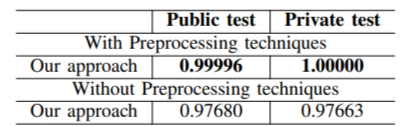
\includegraphics{./pic/2.png}

\section{6.结果}\label{6ux7ed3ux679c}

我们选择在\texttt{AutoDL}平台上进行实验复现。

我们租用了4张3080ti的卡进行训练,训练过程如图:

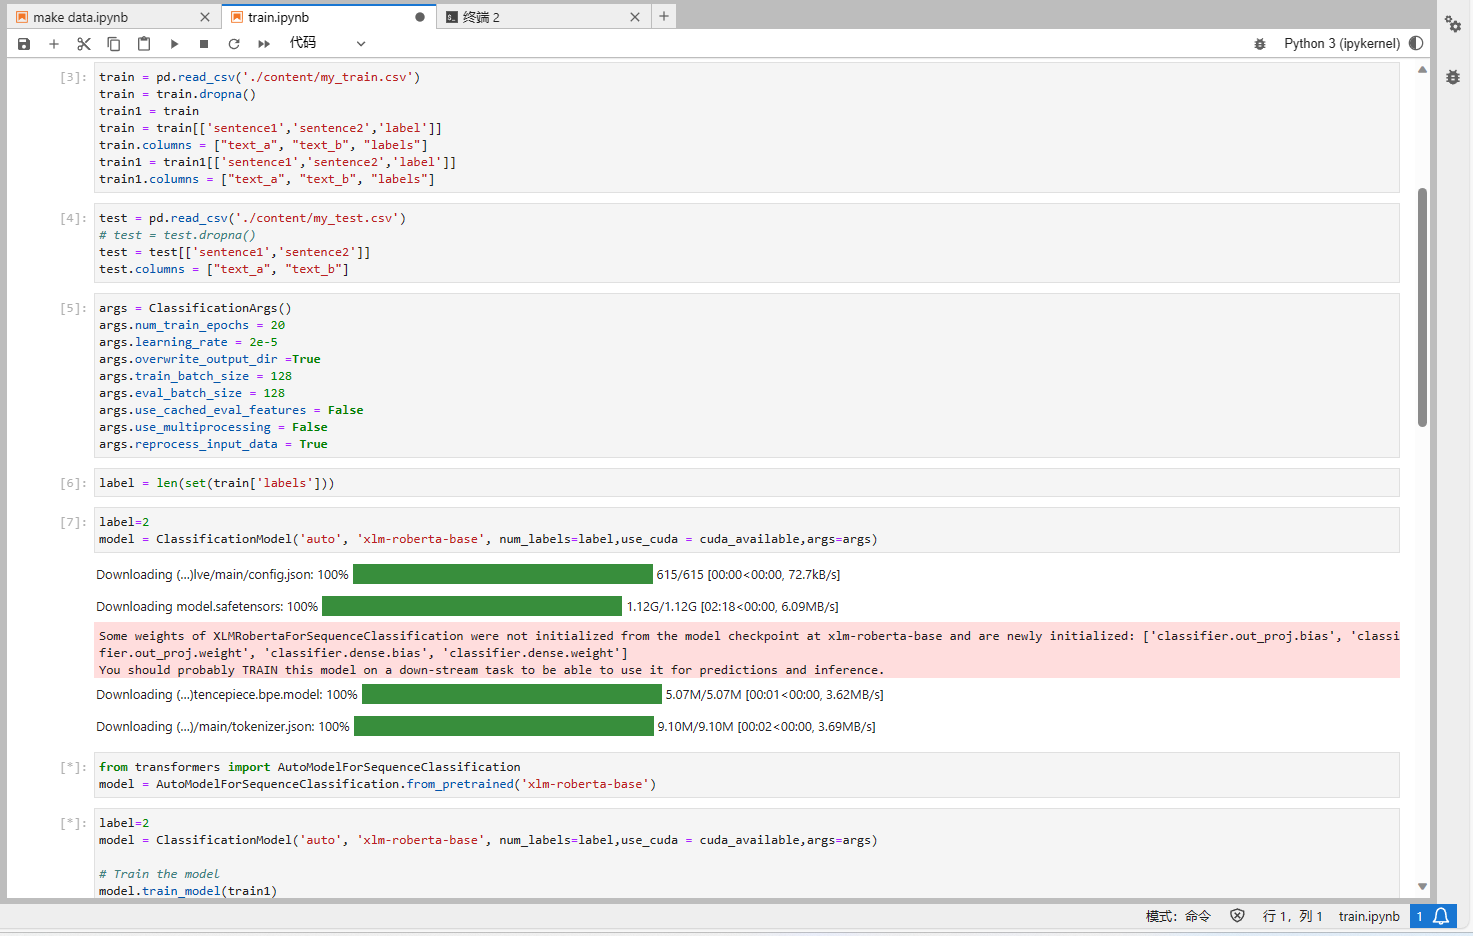
\includegraphics{./pic/3.png}

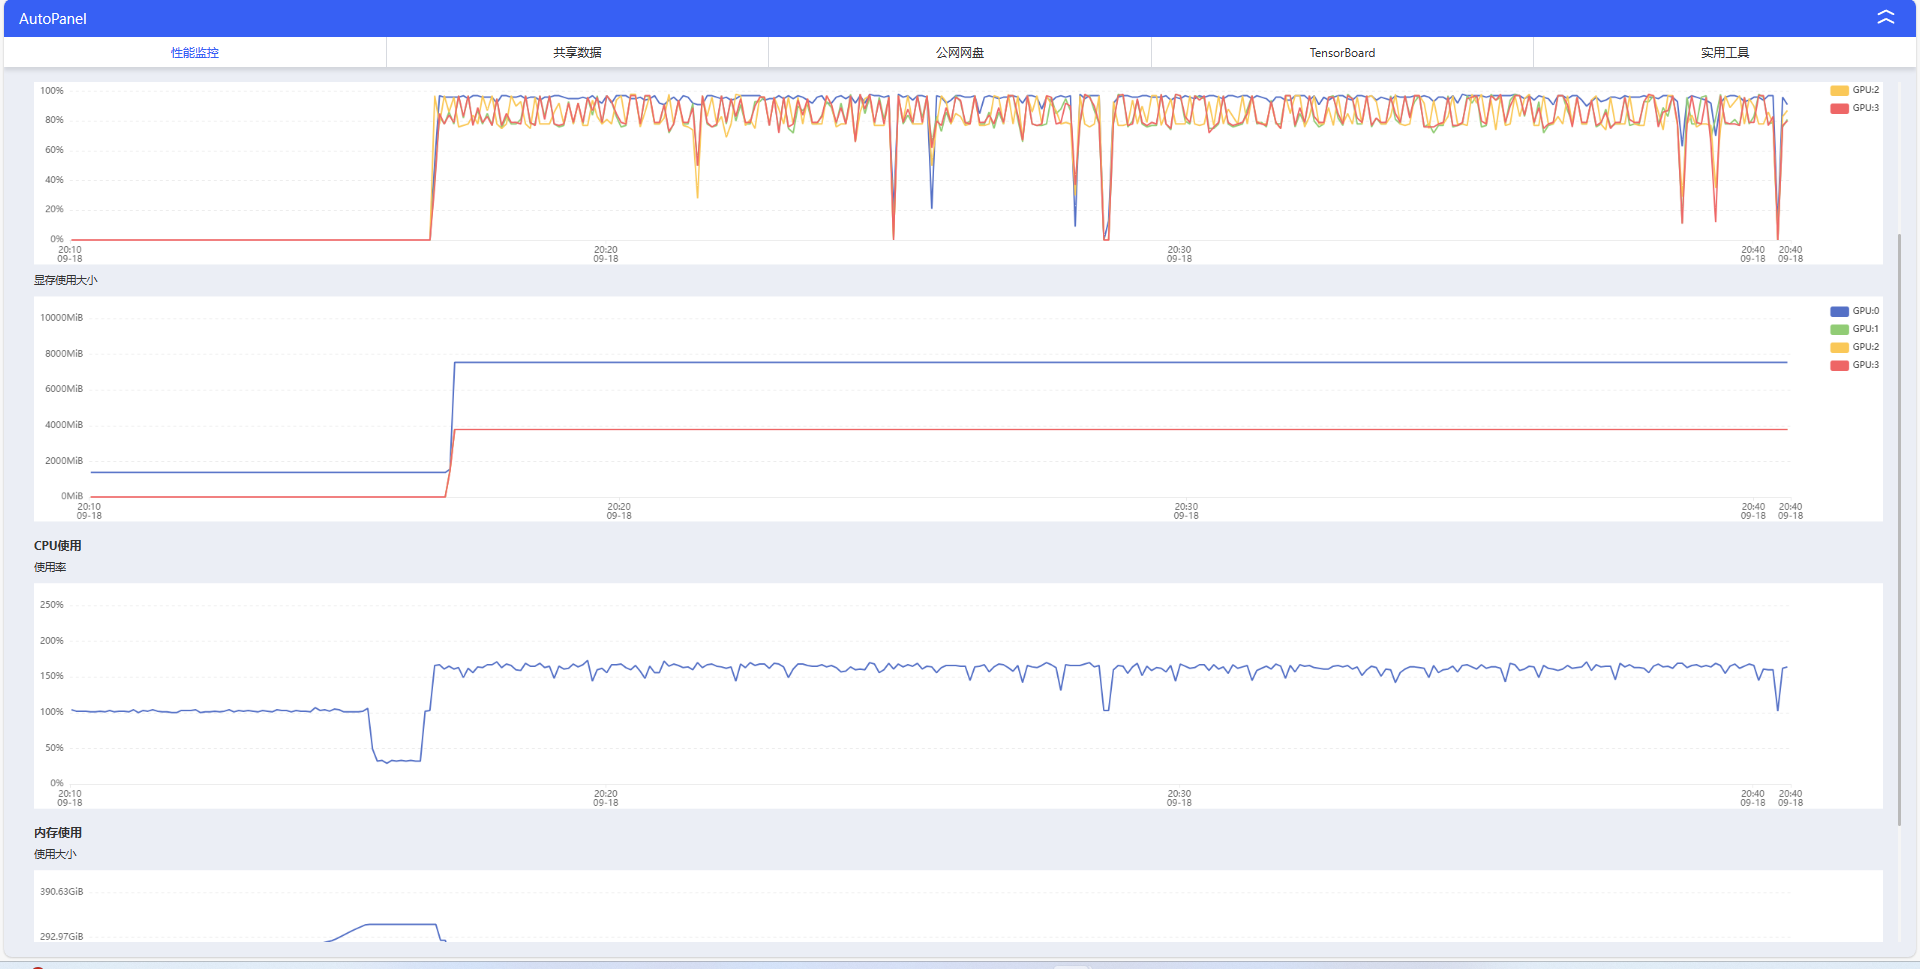
\includegraphics{./pic/4.png}

最终模型评估的结果如下:

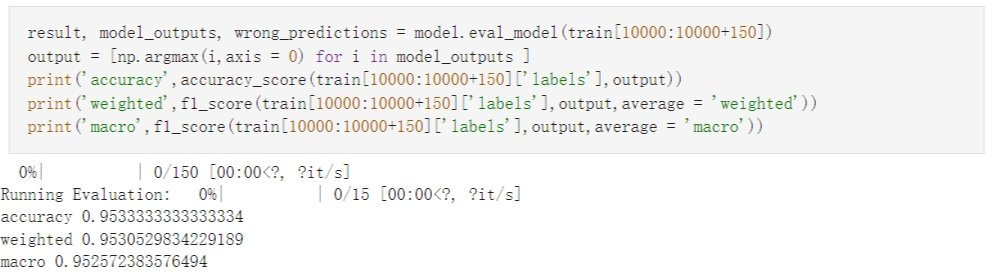
\includegraphics{./pic/5.png}

得到的结果与论文的结果基本相近。碍于算力,训练的模型并未到达文中的最佳效果。

\end{document}
